\documentclass[a4paper,11pt]{jsarticle}


% 数式
\usepackage{amsmath,amsfonts,amssymb}
\usepackage{bm}
% 画像
\usepackage[dvipdfmx]{graphicx}
\usepackage[dvipdfmx]{color}
\usepackage{siunitx}
\usepackage{wrapfig}
\usepackage{cases}
\usepackage{dcolumn}
\usepackage{subcaption}
\makeatletter
\newcommand{\figcaption}[1]{\def\@captype{figure}\caption{#1}}
\newcommand{\tblcaption}[1]{\def\@captype{table}\caption{#1}}
\makeatother

\usepackage{listings,jvlisting}
\lstset{
basicstyle={\ttfamily},
identifierstyle={\small},
commentstyle={\smallitshape},
keywordstyle={\small\bfseries},
ndkeywordstyle={\small},
stringstyle={\small\ttfamily},
frame={tb},
breaklines=true,
columns=[l]{fullflexible},
numbers=left,
xrightmargin=0zw,
xleftmargin=3zw,
numberstyle={\scriptsize},
stepnumber=1,
numbersep=1zw,
lineskip=-0.5ex
}

% 数式の改ページ
\allowdisplaybreaks[1]

\begin{document}

\title{衝突前後の運動方程式について}
\author{平林広}
\date{\today}
\maketitle

今回の文書の目的は
衝突によって物理量の変化が想像しづらい場合において
どのように衝突を考えるべきかをまとめることである.

\section{重力下での煙突方向衝突}
まずは慣れ親しんだ衝突から
加速度や力といった2階微分の物理量以外は衝突において無視してよいことを学ぶ.

\begin{figure}[h]
  \centering
  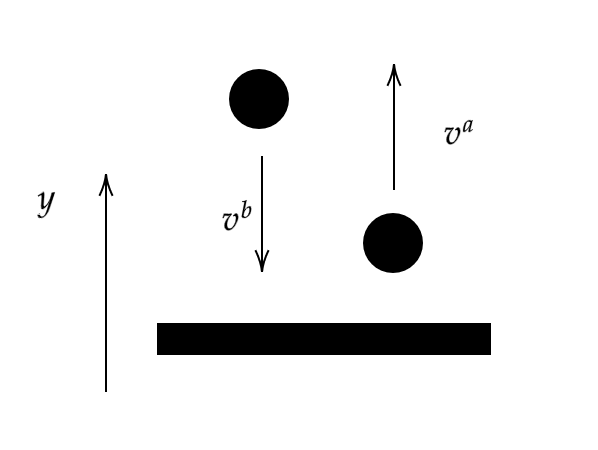
\includegraphics[width = 0.6\textwidth]{ball_freefall.png}
  \caption{衝突状況}
  \label{ball_freefall.png}
\end{figure}

質点$m$が鉛直方向のみに運動し,
地面に速度$v^b (b\text{はbeforeの意図})$ で衝突し,
速度$v^a (a\text{はafterの意図})$で跳ね上がる場合を考える.
ただし,ここで$v^a$は未知である,という考えておく.

衝突は$t=0$で起きるように時刻$t$を取る.
運動方程式は地面からの力を$F$として
\begin{align*}
  m a = -mg + F
\end{align*}
とあらわされる.ただし$F$は以下程度にしか分からない.
\begin{align*}
  F = \begin{cases}
    \infty & (t = 0)
    \\
    0 & (t \neq 0)
  \end{cases}
  .
\end{align*}

区間$[-t_1, t_1]$での積分を考える.
\begin{align*}
  \int_{-t_1}^{t_1} m a dt = \int_{-t_1}^{t_1} -mg dt + \int_{-t_1}^{t_1} F dt
  .
\end{align*}
$t_1 \rightarrow 0$の極限をとれば,$F$による力積を$L$として,
\begin{gather*}
  \int_{-t_1}^{t_1} m a dt \rightarrow m(v^a - v^b),
  \int_{-t_1}^{t_1} -mg dt \rightarrow 0,
  \int_{-t_1}^{t_1} F dt = L
\end{gather*}
となるから,
衝突の前後において
\begin{gather}
  m(v^a - v^b) = L
  \label{case1:newton}
\end{gather}
となる.
しかし現時点では未知数が$v^a, L$に対して,方程式が1つであるため,解けない.

そこで,衝突の条件を考える.
弾性係数を$e$とすると,
\begin{gather}
  v^a = -e v^b
  \label{case1:collision}
\end{gather}
という方程式が導かれる.

よって Equation \ref{case1:newton}, \ref{case1:collision}により
\begin{align*}
  \begin{cases}
    m(v^a - v^b) &= L
    \\
    v^a = -e v^b
  \end{cases}
\end{align*}
と,未知数が$v^a, L$に対して,方程式が2つ成り立つため,
$v^a, L$を決定することができる.

\section{単振り子の衝突}

\begin{figure}[h]
  \centering
  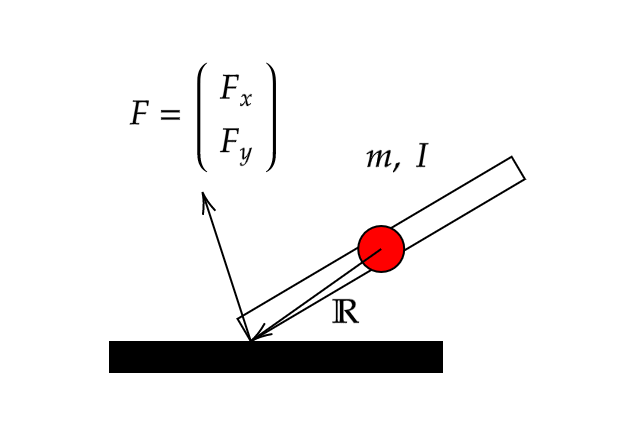
\includegraphics[width = 0.6\textwidth]{1seg_collision.png}
  \caption{単振り子の衝突状況}
  \label{1seg_collision.png}
\end{figure}

次に,衝突後の想像が1段階難しくなる,単振り子の衝突を考える.
何が難しいかというと,端点での衝突によって重心速度が変わることはもちろん,
回転速度$\omega$も変化することが難しい.
そして,端点は質量が0だから,衝突の前後で弾性係数から力積を求めることもできない.

先ほどと同様,beforeのb, afterのa を使って,
衝突前の状態を$v_x^b, v_y^a, \omega^b$,
衝突後の状態を$v_x^a, v_y^a, \omega^a$
とする.
$v_x^a, v_y^a, \omega^a$は全て未知数である.

ニュートンの運動方程式は
\begin{gather*}
  \begin{cases}
    m a_x &= F_x
    \\
    m a_y &= F_y
    \\
    I\dot{\omega} &= \mathbb{R} \times \mathbb{F}
  \end{cases}
\end{gather*}
と表される.
ただし$\mathbb{F}$は
\begin{gather*}
  \mathbb{F} = \begin{pmatrix}
    F_x
    \\
    F_y
  \end{pmatrix}
  = \begin{cases}
    \begin{pmatrix}
      0
      \\
      0
    \end{pmatrix} & (t\neq 0)
    \\
    \begin{pmatrix}
      \infty
      \\
      \infty
    \end{pmatrix} & (t = 0)
  \end{cases}
\end{gather*}
であり,この時点では分からない.

先ほどと同様に
区間$[-t_1, t_1]$での積分の$t_1\rightarrow 0$の極限を考える.
$\mathbb{F}$による力積を$\mathbb{L}$として,
$x$方向について
\begin{gather*}
  \lim_{t_1 \rightarrow 0}\int_{-t_1}^{t_1} m a_x dt = \lim_{t_1 \rightarrow 0}\int_{-t_1}^{t_1} F_x dt = L_x,
  \\
  \Rightarrow
  m (v_x^a - v_x^b) = L_x.
\end{gather*}
$y$方向について
\begin{gather*}
  \lim_{t_1 \rightarrow 0}\int_{-t_1}^{t_1} m a_y dt
  = \lim_{t_1 \rightarrow 0}\int_{-t_1}^{t_1} -mg dt 
  + \lim_{t_1 \rightarrow 0}\int_{-t_1}^{t_1} F_y dt = 0 + L_y
  \\
  \Rightarrow
  m (v_y^a - v_y^b) = L_y.
\end{gather*}
回転について
\begin{align*}
  \lim_{t_1 \rightarrow 0} \int_{-t_1}^{t_1} I\dot\omega dt
  = \lim_{t_1 \rightarrow 0} \int_{-t_1}^{t_1} \mathbb{R} \times \mathbb{F}.
\end{align*}
ここで,極限と積分が入れ替えられることを認めると
\begin{align*}
  \lim_{t_1 \rightarrow 0} \int_{-t_1}^{t_1} I\dot\omega dt
  &= \lim_{t_1 \rightarrow 0} \int_{-t_1}^{t_1} \mathbb{R} \times \mathbb{F}
  \\ &= \mathbb{R} \times \lim_{t_1 \rightarrow 0} \int_{-t_1}^{t_1} \mathbb{F}
  \\ &= \mathbb{R} \times \mathbb{L},
\end{align*}
\begin{gather*}
  \Rightarrow
  I (\omega^a - \omega^b) = \mathbb{R} \times \mathbb{L}.
\end{gather*}
まとめると
\begin{gather*}
  \begin{cases}
    m (v_x^a - v_x^b) = L_x
    \\
    m (v_y^a - v_y^b) = L_y
    \\
    I (\omega^a - \omega^b) = \mathbb{R} \times \mathbb{L}
  \end{cases}
\end{gather*}
であることが分かった.
この時点で$v_x^a, v_y^a, \omega^a, L_x, L_y$が未知数であり,
方程式が3つあるため,2つ足りない状況である.

そこで,衝突の条件を考える.
弾性係数を$e$とすると,
質量が0といっても端点での速度がこの弾性係数に従う.
端点での速度$\mathrm{v}_c (\text{cはcollisionのc})$は
\begin{gather}
  \mathrm{v}_c = \begin{pmatrix}
    v_x
    \\
    v_y
  \end{pmatrix} + \mathbb{R} \times \omega
\end{gather}
によって求められる.
これらが2成分持つことによって残りの2方程式が導かれる.
例えば$x,y$方向のどちらにおいても弾性係数が0の場合は
\begin{gather*}
  \mathrm{v}_c^a = \begin{pmatrix}
    v_x^a
    \\
    v_y^a
  \end{pmatrix} + \mathbb{R} \times \omega^a = \vec{0}
\end{gather*}
という方程式が導かれる.

\clearpage
\section{2重振り子の衝突}

慣れれば衝突は,
\begin{itemize}
  \item 運動方程式から,2回微分以外を含まない項を除き,2回微分を速度変化や力積に入れ替えたもの.
  \item 衝突による速度変化の条件
\end{itemize}
によって簡単に求められる.
運動方程式は実は2回微分の項に関しては1次線形だし,
衝突の条件も基本的に1次線形だから,
行列形式に直して機械的に速度変化や力積を求めることができる.

例えば、
固定軸を持たない2重振り子の片方の端点での衝突を考える
(図 \ref{2seg_collision.png})。
片方の端点での衝突はもう片方の速度、角速度に影響を及ぼすため、少し難しくなる。

\begin{figure}[h]
  \centering
  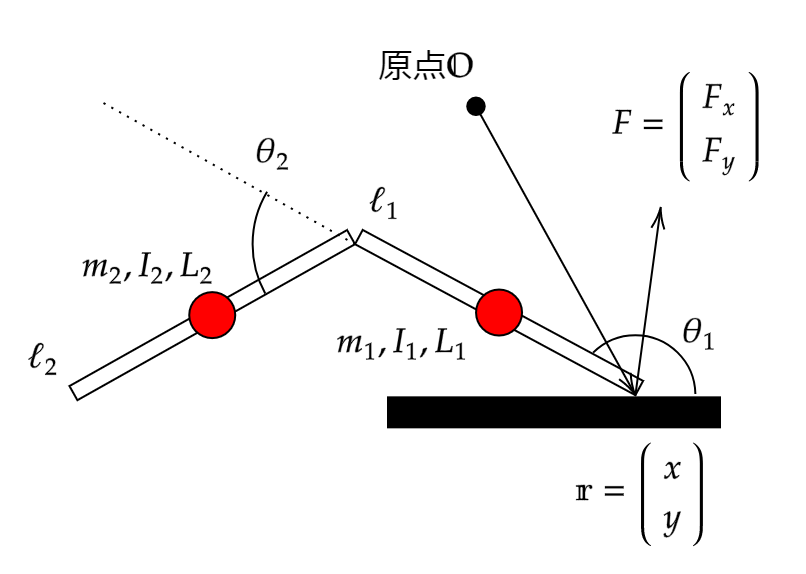
\includegraphics[width = 0.6\textwidth]{2seg_collision.png}
  \caption{固定軸を持たない2重振り子}
  \label{2seg_collision.png}
\end{figure}

この時、$\alpha_1 := \ddot{\theta}_1$は次の難解な方程式を満たす。
\tiny
\begin{align*}
  \alpha_1 =
  &\,\tau _{1} & &
  \\
    & &\times &
    \Bigg(2\,{L_2}^2\,{m_{1}}^2\,m_{2}+2\,{L_2}^2\,m_{1}\,{m_{2}}^2+2\,I_{2}\,{m_{1}}^2+4\,I_{2}\,m_{1}\,m_{2}+2\,I_{2}\,{m_{2}}^2\Bigg)
    \\
    & & &\Bigg/ 
    \Bigg(
      2\,I_{1}\,I_{2}\,{m_{1}}^2+
      2\,I_{1}\,I_{2}\,{m_{2}}^2+
      {\ell_{1}}^2\,{L_2}^2\,{m_{1}}^2\,{m_{2}}^2+
      {L_1}^2\,{L_2}^2\,{m_{1}}^2\,{m_{2}}^2+
      2\,I_{2}\,{\ell_{1}}^2\,m_{1}\,{m_{2}}^2+
      2\,I_{2}\,{\ell_{1}}^2\,{m_{1}}^2\,m_{2}
      \\ & & &+
      2\,I_{1}\,{L_2}^2\,m_{1}\,{m_{2}}^2+
      2\,I_{1}\,{L_2}^2\,{m_{1}}^2\,m_{2}+
      2\,I_{2}\,{L_1}^2\,m_{1}\,{m_{2}}^2+
      2\,I_{2}\,{L_1}^2\,{m_{1}}^2\,m_{2}
      \\ & & &+
      4\,I_{1}\,I_{2}\,m_{1}\,m_{2}-
      2\,\ell_{1}\,L_1\,{L_2}^2\,{m_{1}}^2\,{m_{2}}^2-
      4\,I_{2}\,\ell_{1}\,L_1\,m_{1}\,{m_{2}}^2-
      4\,I_{2}\,\ell_{1}\,L_1\,{m_{1}}^2\,m_{2}
      \\ & & &-
      {\ell_{1}}^2\,{L_2}^2\,{m_{1}}^2\,{m_{2}}^2\,\cos\left(2\,\theta_2\right)-
      {L_1}^2\,{L_2}^2\,{m_{1}}^2\,{m_{2}}^2\,\cos\left(2\,\theta_2\right)+
      2\,\ell_{1}\,L_1\,{L_2}^2\,{m_{1}}^2\,{m_{2}}^2\,\cos\left(2\,\theta_2\right)
    \Bigg)
  \\
  &-\,\tau _{2} & &
  \\
    & & \times &
    \Bigg(
      2\,I_{2}\,{m_{1}}^2+
      2\,I_{2}\,{m_{2}}^2+
      2\,{L_2}^2\,m_{1}\,{m_{2}}^2+
      2\,{L_2}^2\,{m_{1}}^2\,m_{2}+
      4\,I_{2}\,m_{1}\,m_{2}+
      2\,\ell_{1}\,L_2\,m_{1}\,{m_{2}}^2\,\cos\left(\theta_2\right)
      \\ & & &+
      2\,\ell_{1}\,L_2\,{m_{1}}^2\,m_{2}\,\cos\left(\theta_2\right)-
      2\,L_1\,L_2\,m_{1}\,{m_{2}}^2\,\cos\left(\theta_2\right)-
      2\,L_1\,L_2\,{m_{1}}^2\,m_{2}\,\cos\left(\theta_2\right)
    \Bigg)
    \\
    & & &\Bigg/
    \Bigg(
      2\,I_{1}\,I_{2}\,{m_{1}}^2+
      2\,I_{1}\,I_{2}\,{m_{2}}^2+
      {\ell_{1}}^2\,{L_2}^2\,{m_{1}}^2\,{m_{2}}^2+
      {L_1}^2\,{L_2}^2\,{m_{1}}^2\,{m_{2}}^2+
      2\,I_{2}\,{\ell_{1}}^2\,m_{1}\,{m_{2}}^2
      \\ & & &+
      2\,I_{2}\,{\ell_{1}}^2\,{m_{1}}^2\,m_{2}+
      2\,I_{1}\,{L_2}^2\,m_{1}\,{m_{2}}^2+
      2\,I_{1}\,{L_2}^2\,{m_{1}}^2\,m_{2}+
      2\,I_{2}\,{L_1}^2\,m_{1}\,{m_{2}}^2+
      2\,I_{2}\,{L_1}^2\,{m_{1}}^2\,m_{2}
      \\ & & &+
      4\,I_{1}\,I_{2}\,m_{1}\,m_{2}-
      2\,\ell_{1}\,L_1\,{L_2}^2\,{m_{1}}^2\,{m_{2}}^2-
      4\,I_{2}\,\ell_{1}\,L_1\,m_{1}\,{m_{2}}^2-
      4\,I_{2}\,\ell_{1}\,L_1\,{m_{1}}^2\,m_{2}
      \\ & & &-
      {\ell_{1}}^2\,{L_2}^2\,{m_{1}}^2\,{m_{2}}^2\,\cos\left(2\,\theta_2\right)-
      {L_1}^2\,{L_2}^2\,{m_{1}}^2\,{m_{2}}^2\,\cos\left(2\,\theta_2\right)+
      2\,\ell_{1}\,L_1\,{L_2}^2\,{m_{1}}^2\,{m_{2}}^2\,\cos\left(2\,\theta_2\right)
    \Bigg)
  \\
  & +\,\mathrm{Fx} & &
  \\
    & & \times &
    \Bigg(
      2\,I_{2}\,\ell_{1}\,{m_{2}}^2\,\sin\left(\theta_1\right)+
      2\,I_{2}\,L_1\,{m_{1}}^2\,\sin\left(\theta_1\right)+
      \ell_{1}\,{L_2}^2\,m_{1}\,{m_{2}}^2\,\sin\left(\theta_1\right)+
      L_1\,{L_2}^2\,m_{1}\,{m_{2}}^2\,\sin\left(\theta_1\right)
      \\ & & &+
      2\,L_1\,{L_2}^2\,{m_{1}}^2\,m_{2}\,\sin\left(\theta_1\right)+
      2\,I_{2}\,\ell_{1}\,m_{1}\,m_{2}\,\sin\left(\theta_1\right)+
      2\,I_{2}\,L_1\,m_{1}\,m_{2}\,\sin\left(\theta_1\right)
      \\ & & &-
      \ell_{1}\,{L_2}^2\,m_{1}\,{m_{2}}^2\,\sin\left(\theta_1+
      2\,\theta_2\right)+
      L_1\,{L_2}^2\,m_{1}\,{m_{2}}^2\,\sin\left(\theta_1+
      2\,\theta_2\right)
    \Bigg)
    \\
    & & &\Bigg/
    \Bigg(
      2\,I_{1}\,I_{2}\,{m_{1}}^2+
      2\,I_{1}\,I_{2}\,{m_{2}}^2+
      {\ell_{1}}^2\,{L_2}^2\,{m_{1}}^2\,{m_{2}}^2+
      {L_1}^2\,{L_2}^2\,{m_{1}}^2\,{m_{2}}^2
      \\ & & &+
      2\,I_{2}\,{\ell_{1}}^2\,m_{1}\,{m_{2}}^2+
      2\,I_{2}\,{\ell_{1}}^2\,{m_{1}}^2\,m_{2}+
      2\,I_{1}\,{L_2}^2\,m_{1}\,{m_{2}}^2+
      2\,I_{1}\,{L_2}^2\,{m_{1}}^2\,m_{2}+
      2\,I_{2}\,{L_1}^2\,m_{1}\,{m_{2}}^2
      \\ & & &+
      2\,I_{2}\,{L_1}^2\,{m_{1}}^2\,m_{2}+
      4\,I_{1}\,I_{2}\,m_{1}\,m_{2}-
      2\,\ell_{1}\,L_1\,{L_2}^2\,{m_{1}}^2\,{m_{2}}^2-
      4\,I_{2}\,\ell_{1}\,L_1\,m_{1}\,{m_{2}}^2-
      4\,I_{2}\,\ell_{1}\,L_1\,{m_{1}}^2\,m_{2}
      \\ & & &-
      {\ell_{1}}^2\,{L_2}^2\,{m_{1}}^2\,{m_{2}}^2\,\cos\left(2\,\theta_2\right)-
      {L_1}^2\,{L_2}^2\,{m_{1}}^2\,{m_{2}}^2\,\cos\left(2\,\theta_2\right)+
      2\,\ell_{1}\,L_1\,{L_2}^2\,{m_{1}}^2\,{m_{2}}^2\,\cos\left(2\,\theta_2\right)
    \Bigg)
  \\
  & -\,\mathrm{Fy} & &
  \\
    & & \times &
    \Bigg(
        2\,I_{2}\,\ell_{1}\,{m_{2}}^2\,\cos\left(\theta_1\right)+
        2\,I_{2}\,L_1\,{m_{1}}^2\,\cos\left(\theta_1\right)+
        \ell_{1}\,{L_2}^2\,m_{1}\,{m_{2}}^2\,\cos\left(\theta_1\right)
        \\ & & &+
        L_1\,{L_2}^2\,m_{1}\,{m_{2}}^2\,\cos\left(\theta_1\right)+
        2\,L_1\,{L_2}^2\,{m_{1}}^2\,m_{2}\,\cos\left(\theta_1\right)+
        2\,I_{2}\,\ell_{1}\,m_{1}\,m_{2}\,\cos\left(\theta_1\right)
        \\ & & &+
        2\,I_{2}\,L_1\,m_{1}\,m_{2}\,\cos\left(\theta_1\right)-
        \ell_{1}\,{L_2}^2\,m_{1}\,{m_{2}}^2\,\cos\left(\theta_1+
        2\,\theta_2\right)+
        L_1\,{L_2}^2\,m_{1}\,{m_{2}}^2\,\cos\left(\theta_1+
        2\,\theta_2\right)
    \Bigg)
    \\
    & & &\Bigg/ 
    \Bigg(
      2\,I_{1}\,I_{2}\,{m_{1}}^2+
      2\,I_{1}\,I_{2}\,{m_{2}}^2+
      {\ell_{1}}^2\,{L_2}^2\,{m_{1}}^2\,{m_{2}}^2+
      {L_1}^2\,{L_2}^2\,{m_{1}}^2\,{m_{2}}^2
      \\ & & &+
      2\,I_{2}\,{\ell_{1}}^2\,m_{1}\,{m_{2}}^2+
      2\,I_{2}\,{\ell_{1}}^2\,{m_{1}}^2\,m_{2}+
      2\,I_{1}\,{L_2}^2\,m_{1}\,{m_{2}}^2+
      2\,I_{1}\,{L_2}^2\,{m_{1}}^2\,m_{2}+
      2\,I_{2}\,{L_1}^2\,m_{1}\,{m_{2}}^2
      \\ & & &+
      2\,I_{2}\,{L_1}^2\,{m_{1}}^2\,m_{2}+
      4\,I_{1}\,I_{2}\,m_{1}\,m_{2}-
      2\,\ell_{1}\,L_1\,{L_2}^2\,{m_{1}}^2\,{m_{2}}^2-
      4\,I_{2}\,\ell_{1}\,L_1\,m_{1}\,{m_{2}}^2-
      4\,I_{2}\,\ell_{1}\,L_1\,{m_{1}}^2\,m_{2}
      \\ & & &-
      {\ell_{1}}^2\,{L_2}^2\,{m_{1}}^2\,{m_{2}}^2\,\cos\left(2\,\theta_2\right)-
      {L_1}^2\,{L_2}^2\,{m_{1}}^2\,{m_{2}}^2\,\cos\left(2\,\theta_2\right)+
      2\,\ell_{1}\,L_1\,{L_2}^2\,{m_{1}}^2\,{m_{2}}^2\,\cos\left(2\,\theta_2\right)
    \Bigg)
  \\
  & + & &
  \\
    & & &\Bigg(
      \sin\left(2\,\theta_2\right)\,{\ell_{1}}^2\,{L_2}^2\,{m_{1}}^2\,{m_{2}}^2\,{\omega _{1}}^2-
      2\,\sin\left(2\,\theta_2\right)\,\ell_{1}\,L_1\,{L_2}^2\,{m_{1}}^2\,{m_{2}}^2\,{\omega _{1}}^2
      \\ & & &+
      2\,\sin\left(\theta_2\right)\,\ell_{1}\,{L_2}^3\,{m_{1}}^2\,{m_{2}}^2\,{\omega _{1}}^2+
      4\,\sin\left(\theta_2\right)\,\ell_{1}\,{L_2}^3\,{m_{1}}^2\,{m_{2}}^2\,\omega _{1}\,\omega _{2}+
      2\,\sin\left(\theta_2\right)\,\ell_{1}\,{L_2}^3\,{m_{1}}^2\,{m_{2}}^2\,{\omega _{2}}^2
      \\ & & &+
      2\,I_{2}\,\sin\left(\theta_2\right)\,\ell_{1}\,L_2\,{m_{1}}^2\,m_{2}\,{\omega _{1}}^2+
      4\,I_{2}\,\sin\left(\theta_2\right)\,\ell_{1}\,L_2\,{m_{1}}^2\,m_{2}\,\omega _{1}\,\omega _{2}+
      2\,I_{2}\,\sin\left(\theta_2\right)\,\ell_{1}\,L_2\,{m_{1}}^2\,m_{2}\,{\omega _{2}}^2
      \\ & & &+
      2\,I_{2}\,\sin\left(\theta_2\right)\,\ell_{1}\,L_2\,m_{1}\,{m_{2}}^2\,{\omega _{1}}^2+
      4\,I_{2}\,\sin\left(\theta_2\right)\,\ell_{1}\,L_2\,m_{1}\,{m_{2}}^2\,\omega _{1}\,\omega _{2}+
      2\,I_{2}\,\sin\left(\theta_2\right)\,\ell_{1}\,L_2\,m_{1}\,{m_{2}}^2\,{\omega _{2}}^2
      \\ & & &+
      \sin\left(2\,\theta_2\right)\,{L_1}^2\,{L_2}^2\,{m_{1}}^2\,{m_{2}}^2\,{\omega _{1}}^2
      \\ & & &-
      2\,\sin\left(\theta_2\right)\,L_1\,{L_2}^3\,{m_{1}}^2\,{m_{2}}^2\,{\omega _{1}}^2-
      4\,\sin\left(\theta_2\right)\,L_1\,{L_2}^3\,{m_{1}}^2\,{m_{2}}^2\,\omega _{1}\,\omega _{2}-
      2\,\sin\left(\theta_2\right)\,L_1\,{L_2}^3\,{m_{1}}^2\,{m_{2}}^2\,{\omega _{2}}^2
      \\ & & &-
      2\,I_{2}\,\sin\left(\theta_2\right)\,L_1\,L_2\,{m_{1}}^2\,m_{2}\,{\omega _{1}}^2-
      4\,I_{2}\,\sin\left(\theta_2\right)\,L_1\,L_2\,{m_{1}}^2\,m_{2}\,\omega _{1}\,\omega _{2}-
      2\,I_{2}\,\sin\left(\theta_2\right)\,L_1\,L_2\,{m_{1}}^2\,m_{2}\,{\omega _{2}}^2
      \\ & & &-
      2\,I_{2}\,\sin\left(\theta_2\right)\,L_1\,L_2\,m_{1}\,{m_{2}}^2\,{\omega _{1}}^2-
      4\,I_{2}\,\sin\left(\theta_2\right)\,L_1\,L_2\,m_{1}\,{m_{2}}^2\,\omega _{1}\,\omega _{2}-
      2\,I_{2}\,\sin\left(\theta_2\right)\,L_1\,L_2\,m_{1}\,{m_{2}}^2\,{\omega _{2}}^2
    \Bigg)
    \\
    & & &\Bigg/ \Bigg(
      2\,I_{1}\,I_{2}\,{m_{1}}^2+
      2\,I_{1}\,I_{2}\,{m_{2}}^2+
      {\ell_{1}}^2\,{L_2}^2\,{m_{1}}^2\,{m_{2}}^2+
      {L_1}^2\,{L_2}^2\,{m_{1}}^2\,{m_{2}}^2
      \\ & & &+
      2\,I_{2}\,{\ell_{1}}^2\,m_{1}\,{m_{2}}^2+
      2\,I_{2}\,{\ell_{1}}^2\,{m_{1}}^2\,m_{2}+
      2\,I_{1}\,{L_2}^2\,m_{1}\,{m_{2}}^2+
      2\,I_{1}\,{L_2}^2\,{m_{1}}^2\,m_{2}+
      2\,I_{2}\,{L_1}^2\,m_{1}\,{m_{2}}^2+
      2\,I_{2}\,{L_1}^2\,{m_{1}}^2\,m_{2}
      \\ & & &+
      4\,I_{1}\,I_{2}\,m_{1}\,m_{2}-
      2\,\ell_{1}\,L_1\,{L_2}^2\,{m_{1}}^2\,{m_{2}}^2-
      4\,I_{2}\,\ell_{1}\,L_1\,m_{1}\,{m_{2}}^2-
      4\,I_{2}\,\ell_{1}\,L_1\,{m_{1}}^2\,m_{2}
      \\ & & &-
      {\ell_{1}}^2\,{L_2}^2\,{m_{1}}^2\,{m_{2}}^2\,\cos\left(2\,\theta_2\right)-
      {L_1}^2\,{L_2}^2\,{m_{1}}^2\,{m_{2}}^2\,\cos\left(2\,\theta_2\right)+
      2\,\ell_{1}\,L_1\,{L_2}^2\,{m_{1}}^2\,{m_{2}}^2\,\cos\left(2\,\theta_2\right)
    \Bigg)
\end{align*}
\normalsize
他の2回微分である$\alpha_2, a_x, a_y$も同様に難解な方程式を満たすが、
それぞれの係数を適当に置けばこれらを単純に書き直せる。
\begin{align*}
  \alpha_1 &= A_1 \tau_1 + A_2 \tau_2 + A_3 F_x + A_4 F_y + A_5
  \\
  \alpha_2 &= B_1 \tau_1 + B_2 \tau_2 + B_3 F_x + B_4 F_y + B_5
  \\
  a_x &= C_1 \tau_1 + C_2 \tau_2 + C_3 F_x + C_4 F_y + C_5
  \\
  a_y &= D_1 \tau_1 + D_2 \tau_2 + D_3 F_x + D_4 F_y + D_5
\end{align*}
行列形式で表現すると
\begin{align*}
  \begin{pmatrix}
    \alpha_1
    \\
    \alpha_2
    \\
    a_x
    \\
    a_y
  \end{pmatrix}
  =
  \begin{pmatrix}
    A_1 & A_2 & A_3 & A_4
    \\
    B_1 & B_2 & B_3 & B_4
    \\
    C_1 & C_2 & C_3 & C_4
    \\
    D_1 & D_2 & D_3 & D_4
  \end{pmatrix}
  \begin{pmatrix}
    \tau_1
    \\
    \tau_2
    \\
    F_x
    \\
    F_y
  \end{pmatrix}
  + 
  \begin{pmatrix}
    A_5
    \\
    B_5
    \\
    C_5
    \\
    D_5
  \end{pmatrix}
\end{align*}

今までの衝突のように衝突の微小時間に着目すれば
右辺は$\int F_x, \int F_y$のみが残り、
\begin{align*}
  \begin{pmatrix}
    \omega_1^a - \omega_1^b
    \\
    \omega_2^a - \omega_2^b
    \\
    v_x^a - v_x^b
    \\
    v_y^a - v_y^b
  \end{pmatrix}
  =
  \begin{pmatrix}
    A_1 & A_2 & A_3 & A_4
    \\
    B_1 & B_2 & B_3 & B_4
    \\
    C_1 & C_2 & C_3 & C_4
    \\
    D_1 & D_2 & D_3 & D_4
  \end{pmatrix}
  \begin{pmatrix}
    0
    \\
    0
    \\
    \int F_x
    \\
    \int F_y
  \end{pmatrix}
\end{align*}
となる。
ここで未知数は$\omega_1^a, \omega_2^a, v_x^a, v_y^a, \int F_x, \int F_y$の6つで、
方程式はまだ4つしか見つかっていない。

そこで衝突の条件として
例えば弾性衝突を考えれば
\begin{align*}
  \begin{cases}
    v_x^a = -v_x^b
    \\
    v_y^a = -v_y^b
  \end{cases}
\end{align*}
の2つの方程式が加わり、未知数が全て求まるようになる。


\end{document}
